\documentclass[11pt,a4paper]{report}
\usepackage[spanish,es-nodecimaldot]{babel}	% Utilizar español
\usepackage[utf8]{inputenc}					% Caracteres UTF-8
\usepackage{graphicx}						% Imagenes
\usepackage[hidelinks]{hyperref}			% Poner enlaces sin marcarlos en rojo
\usepackage{fancyhdr}						% Modificar encabezados y pies de pagina
\usepackage{float}							% Insertar figuras
\usepackage[textwidth=390pt]{geometry}		% Anchura de la pagina
\usepackage[nottoc]{tocbibind}				% Referencias (no incluir num pagina indice en Indice)
\usepackage{enumitem}						% Permitir enumerate con distintos simbolos
\usepackage[T1]{fontenc}					% Usar textsc en sections
\usepackage{amsmath}						% Símbolos matemáticos

% Comando para poner el nombre de la asignatura
\newcommand{\asignatura}{Simulación de Sistemas}
\newcommand{\autor}{Adrián Acosa Sánchez}
\newcommand{\titulo}{PROBLEMA DE MODELO DISCRETO}
\newcommand{\subtitulo}{Problema de las líneas telefónicas}
\newcommand{\rama}{Computación y Sistemas Inteligentes}

% Configuracion de encabezados y pies de pagina
\pagestyle{fancy}
\lhead{\autor{}}
\rhead{\asignatura{}}
\lfoot{Grado en Ingeniería Informática}
\cfoot{}
\rfoot{\thepage}
\renewcommand{\headrulewidth}{0.4pt}		% Linea cabeza de pagina
\renewcommand{\footrulewidth}{0.4pt}		% Linea pie de pagina

\usepackage{graphicx}
\begin{document}
\pagenumbering{gobble}

% Pagina de titulo
\begin{titlepage}

\begin{minipage}{\textwidth}

\centering

%
\includegraphics[scale=0.5]{img/ugr.png}\\

\includegraphics[scale=0.3]{img/logo_ugr.jpg}\\[1cm]

\textsc{\Large \asignatura{}\\[0.2cm]}
\textsc{GRADO EN INGENIERÍA INFORMÁTICA}\\[1cm]

\noindent\rule[-1ex]{\textwidth}{1pt}\\[1.5ex]
\textsc{{\Huge \titulo\\[0.5ex]}}
\textsc{{\Large \subtitulo\\}}
\noindent\rule[-1ex]{\textwidth}{2pt}\\[3.5ex]

\end{minipage}

%\vspace{0.5cm}
\vspace{0.7cm}

\begin{minipage}{\textwidth}

\centering

\textbf{Autor}\\ {\autor{}}\\[2.5ex]
\textbf{Rama}\\ {\rama}\\[2.5ex]
\vspace{0.3cm}


\includegraphics[scale=0.3]{img/etsiit.jpeg}

\vspace{0.7cm}
\textsc{Escuela Técnica Superior de Ingenierías Informática y de Telecomunicación}\\
\vspace{1cm}
\textsc{Curso 2022-2023}
\end{minipage}
\end{titlepage}

\pagenumbering{arabic}
\tableofcontents
\thispagestyle{empty}				% No usar estilo en la pagina de indice

\newpage

\setlength{\parskip}{1em}

\chapter{Problema de modelo discreto}

\newpage

\section{Descripción del problema}

Entre dos ciudades, A y B, existe un número n de líneas telefónicas. Cada línea puede operar en cualquier dirección (llamadas originadas en A o en B), pero sólo admite una llamada al mismo tiempo. Si una persona en A o B quiere hacer una llamada a la otra ciudad y hay una línea abierta (libre), la llamada se efectua inmediatamente a través de alguna de las líneas abiertas. Si las n líneas están ocupadas, se escucha una grabación indicando que se cuelgue y se intente más tarde (no hay posibilidad de retener la llamada y esperar a que una línea quede abierta), de modo que esa llamada se pierde. Los tiempos entre intentos de llamada se distribuyen exponencialmente con media 12 segundos para llamadas de A a B, y de 10 segundos para llamadas de B a A. La duración de la conversación se distribuye exponencialmente con media 4 minutos para ambos tipos de llamadas. Inicialmente todas las líneas están abiertas, y se quiere simular el sistema durante 12 horas.

\section{Planteamiento de la solución}

Para plantear la simulación, en lo primero que nos tenemos que fijar es en qué sucesos existen:

\begin{itemize}
	\item{Inicio}
	\item{Llamada de A a B}
	\item{Llamada de B a A}
	\item{Fin de la simulación}
\end{itemize}

Para cada suceso habrá que programar su rutina, pero antes tenmos que plantear cómo vamos a estructurar los sucesos. Para ello, yo me he basado en el programa dado en la Práctica 3 de múltiples trabajadores y un operario y lo he adaptado al problema que se nos plantea.

Lo indispensable antes de empezar a programar cada una de las rutinas para los sucesos es declarar el generador de los tiempos de llamada, que consistirá en un generador exponencial como se nos indica en el enunciado a la cual le vamos a pasar la media de los tiempos de llamada. De esta forma podemos usarlo tanto para generar las llegadas de las llamadas como para generar los tiempos que duran las llamadas.

Para representar los sucesos lo que haremos será usar una lista de un tipo de dato \texttt{suceso} que tendrá los siguientes campos:

\begin{itemize}
	\item{Tipo de suceso}
	\item{Duracion del suceso}
\end{itemize}

En esta lista de sucesos se irán insertando todos los sucesos que se vayan ordenando en orden creciente de duración del suceso. De esta forma, el primer suceso de la lista será el que se va a ejecutar en el siguiente instante de tiempo.

La manera en la que diferenciamos los sucesos que hay que ejecutar lo haremos con una rutina que se llamara \texttt{suceso}, la cual leerá de la lista de sucesos el primer suceso y verá de qué tipo es. Dependiendo del tipo de suceso que sea, ejecutará una rutina u otra lo cual lo realizaremos con un \texttt{switch}. 

Antes de ejecutar cualquier rutina, lo necesitamos inicializar todas las variables necesarias, lo cual lo haremos con la función \texttt{inicializacion}.

La rutina de llamada es la más importante. Es la rutina que simulará la realización de las llamadas, tanto de A a B como de B a A. Para diferenciar el sentido de la llamada, lo que vamos a hacer es pasarle una media que irá en funcion del suceso que se esté ejecutando. De esta forma, si el suceso es de llamada de A a B, la media que le pasaremos será la de 12 segundos, y si es de B a A, la media será la de 10 segundos.

La rutina de llamada lo que hará será generar el tiempo de llamada, y si hay alguna línea libre, se realizará la llamada. Si no hay ninguna línea libre, se cuelga la llamada. En cualquier caso, se generará el tiempo de la siguiente llamada y se insertará en la lista de sucesos.

La rutina de finalización de llamada vendrá dada por la funcion \texttt{fin\_llamada} la cual lo que hará será simplemente avanzar los contadores de número de llamadas realizadas y el de las líneas libres.

La rutina del fin de la simulación lo único que va a hacer es poner una variable booleana a \texttt{true} para indicar que la simulación ha terminado. Además, llevará la cuenta de las variables estadísticas que se piden en el enunciado.

Con todo esto ya podemos ver la simulación en sí, que consiste en lo mismo que en el problema de Montecarlo: un bucle doble donde el bucle interno será el encargado de la simulación de las 12 horas indicadas (43200 segundos) y el bucle externo será el encargado de ejecutar la simulación n veces para obtener la media de los resultados.

Por último, para poder ver 

\section{Grafo de sucesos}

\begin{figure}[H]
\centering
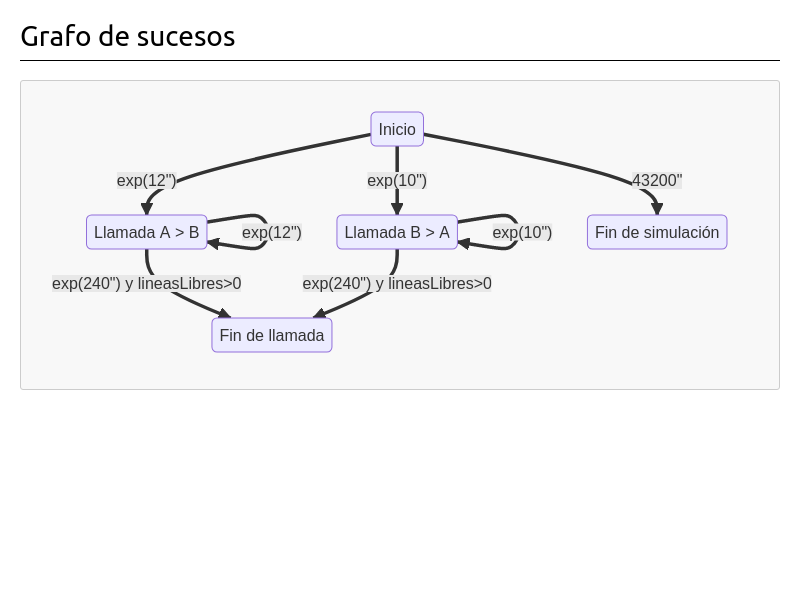
\includegraphics[width=\textwidth]{img/grafo_sucesos.png}
\caption{Grafo de sucesos del modelo}
\label{}
\end{figure}

\section{Resultados}

Todas las simulaciones realizadas a partir de ahora se repetirán 1000 veces. Vamos a probar experimentalmente cuántas líneas telefónicas son necesarias para que las llamadas perdidas sean menos de un 5\%. Comenzaremos con 40 líneas telefónicas, lo que nos da el siguiente resultado:

\begin{itemize}
	\item{Numero medio de lineas ocupadas: 35.059}
	\item{Porcentaje medio de lineas ocupadas: 87.6475\%}
	\item{Numero medio de llamadas atendidas: 6439.31}
	\item{Numero medio de llamadas perdidas: 1030.16}
	\item{Porcentaje medio de llamadas perdidas: 16.0031\%}
\end{itemize}

Como podemos ver, con 40 líneas telefónicas vemos que perdemos un 16\% de las llamadas. Vamos a probar ahora con 60:


\begin{itemize}
	\item{Numero medio de lineas ocupadas: 41.3497}
	\item{Porcentaje medio de lineas ocupadas: 68.9162\%}
	\item{Numero medio de llamadas atendidas: 7451.84}
	\item{Numero medio de llamadas perdidas: 13.296}
	\item{Porcentaje medio de llamadas perdidas: 0.178094\%}
\end{itemize}

Se puede apreciar como añadiendo 20 líneas telefónicas, el porcentaje de llamadas perdidas se reduce a un 0.17\%. Y si ampliamos 15 más tendríamos los siguientes resultados:

\begin{itemize}
	\item{Numero medio de lineas ocupadas: 41.4825}
	\item{Porcentaje medio de lineas ocupadas: 55.31\%}
	\item{Numero medio de llamadas atendidas: 7468.87}
	\item{Numero medio de llamadas perdidas: 0.007}
	\item{Porcentaje medio de llamadas perdidas: $9.29361 * 10^{-5}$\%}
\end{itemize}

Tendríamos prácticamente 0 llamadas perdidas.



\end{document}

